

\subsection{Comparación}

% E- Módulo de evaluación
% - Objetivo del módulo			
% - Explicación básica de la evaluación y comparación de rendimiento de los algoritmos

Por ultimo, podemos comparar los resultados de distintas ejecuciones. La diferencia de las ejecuciones puede estar el algoritmo utilizado para estimar, sin embargo también puede estar en los modelos de trayectoria, en la simulación de señales, o simplemente la frecuencia de muestreo de alguna señal. Debido a que al final del ciclo, navindoor crea trayectorias a partir de las estimaciones, las comparaciones se puede realizar entre dos estimaciones o entre la estimación y la trayectoria real. Un ejemplo de uso pordemos ve en la figura (figura \ref{fig:interfaz5}). 

\begin{figure}
    \centering
    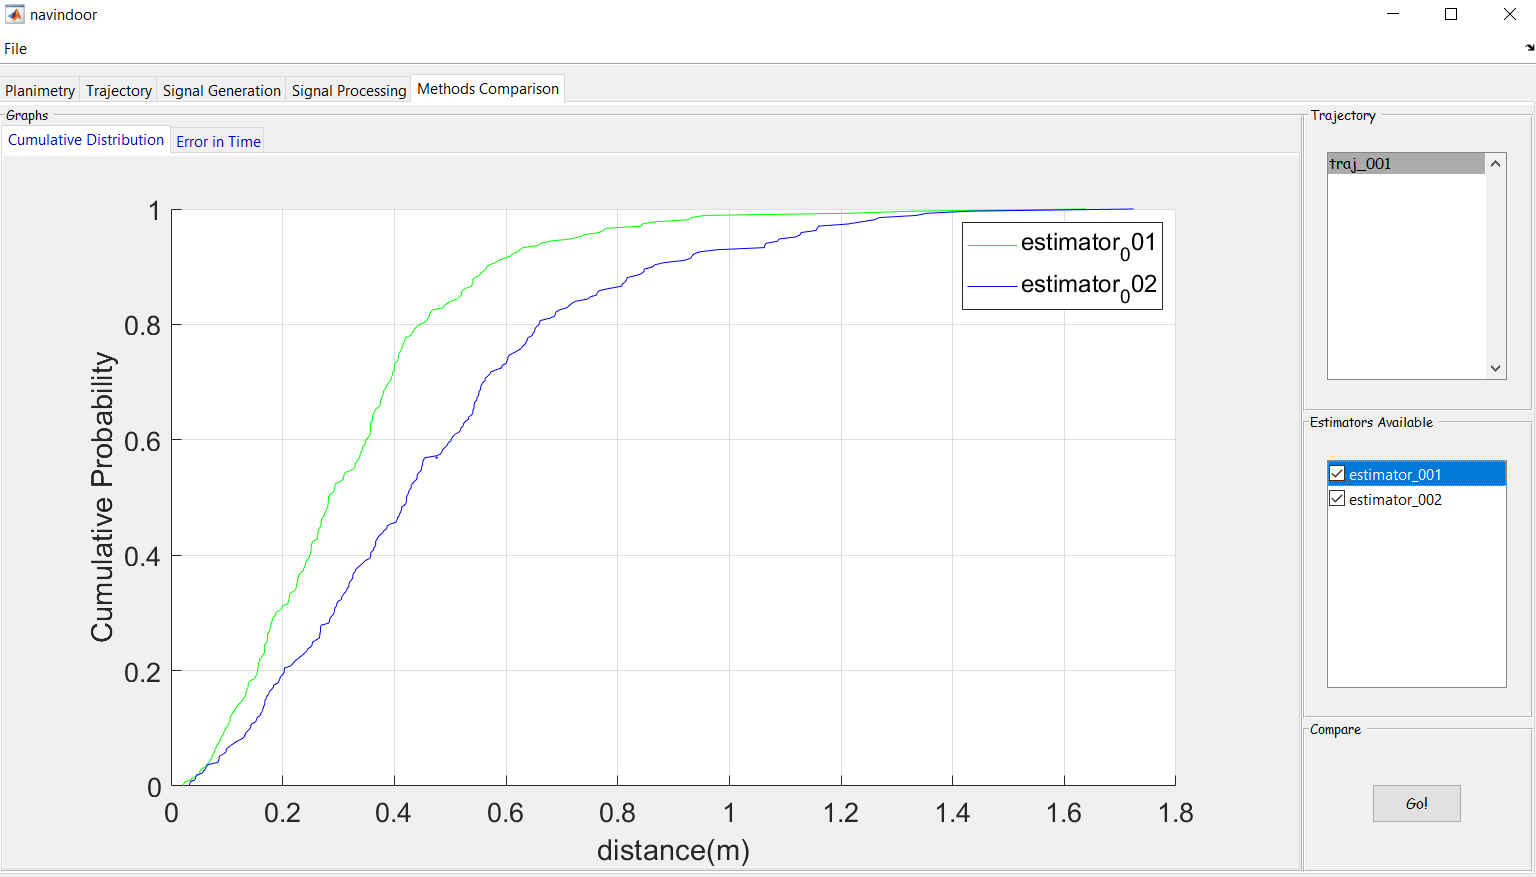
\includegraphics[width=0.8\columnwidth]{img/Design/5.PNG}
    \caption[]{Interfaz gráfica para la comparación de estimaciones.}
    \label{fig:interfaz5}
    \footnotesize 
    En este caso podemos ver el efecto de la frecuencia de muestreo en nuestras estimaciones. La estimación azul se ha realizado con una señal RSS de frecuencia 1Hz, mientras que la ver se ha realizado con una frecuencia de 5Hz.
\end{figure}
